\documentclass[a4paper,10pt]{article}
\usepackage[utf8]{inputenc}
\usepackage{listings}
\usepackage{graphicx}
\usepackage{caption}
\usepackage{subcaption}

%opening
\title{arduino}
\author{---}

\begin{document}

\maketitle

\begin{abstract}

\end{abstract}

\section{Materials (so far)}

\begin{itemize}
 \item Arduino UNO board
 \item Motor shields x2
 \item 9V batteries x2
 \item Stepper DC motor x2
\end{itemize}

\section{Set up}

The Arduino UNO board is unable to provide a high enough voltage to power the motors. Instead, each of the motors is powered by a motor shield (reference)
and powered by a 9V battery. The shields have to be stacked and are mounted on top of the Arduino board. 

\subsection{Boards}

\begin{figure}
    \centering
    \begin{subfigure}[b]{0.32\textwidth}
      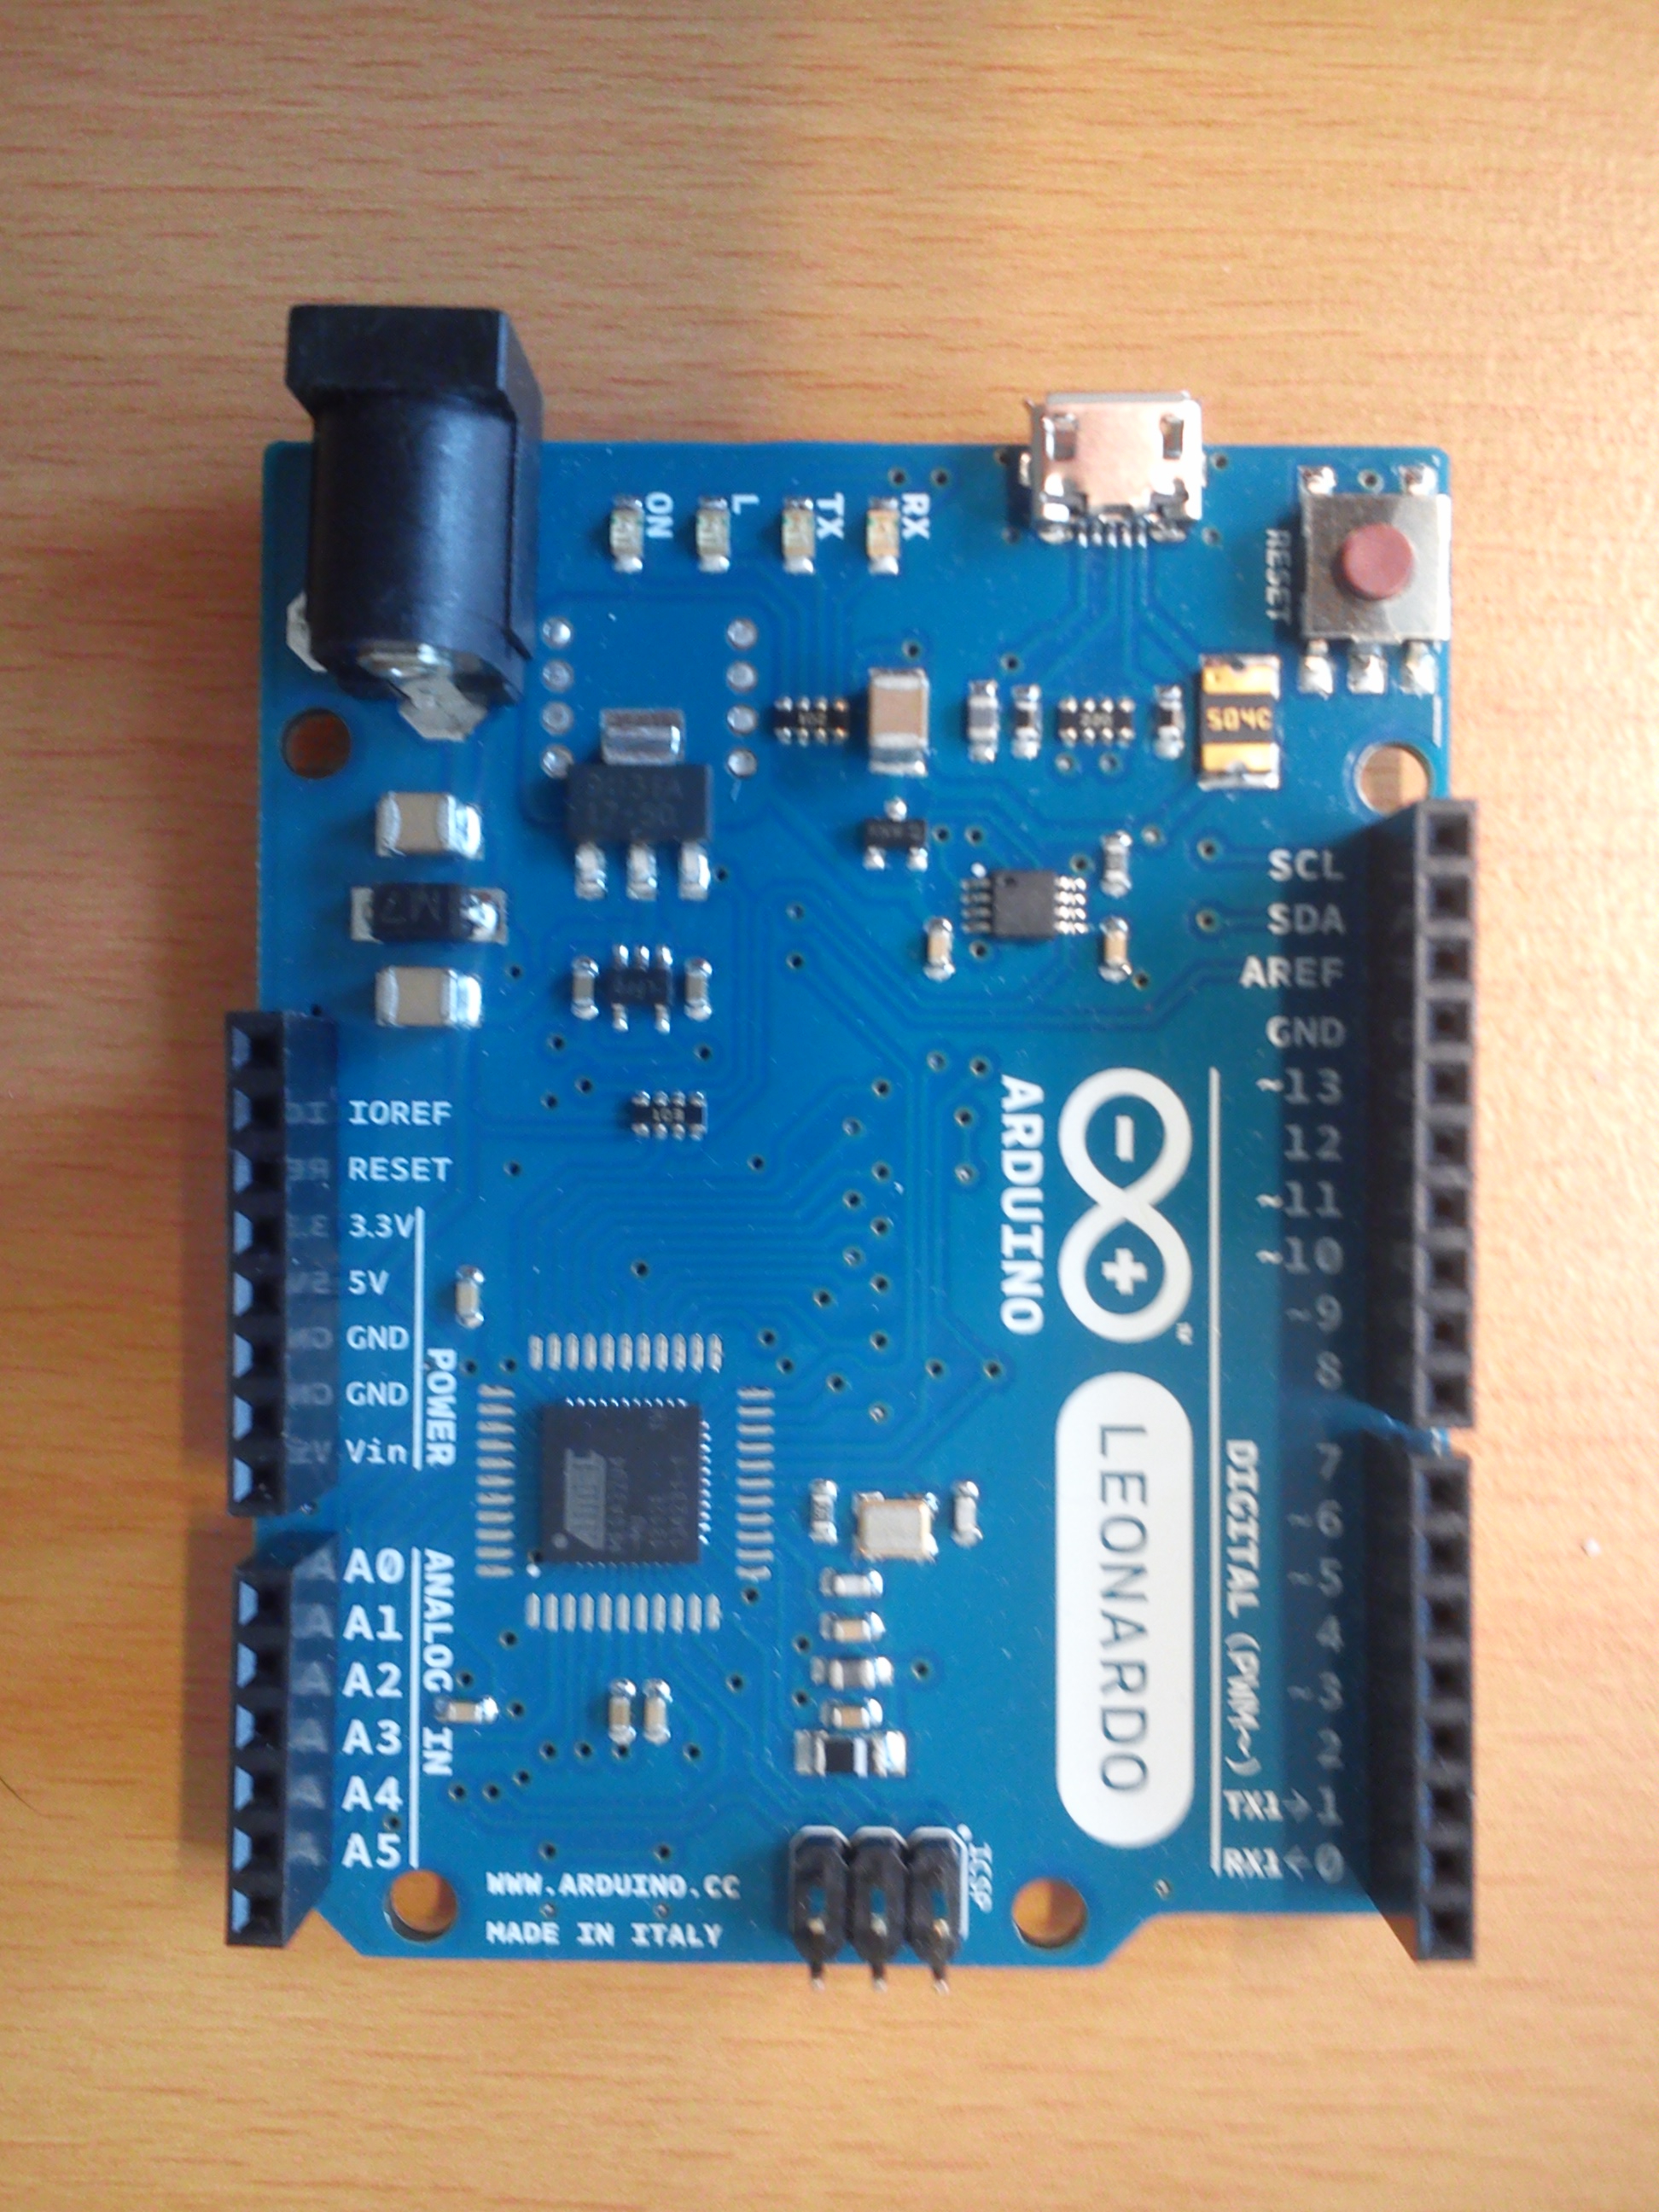
\includegraphics[width=\textwidth]{../figures/leo.jpg}
	  \caption{Arduino board}
    \end{subfigure}
    \begin{subfigure}[b]{0.32\textwidth}
      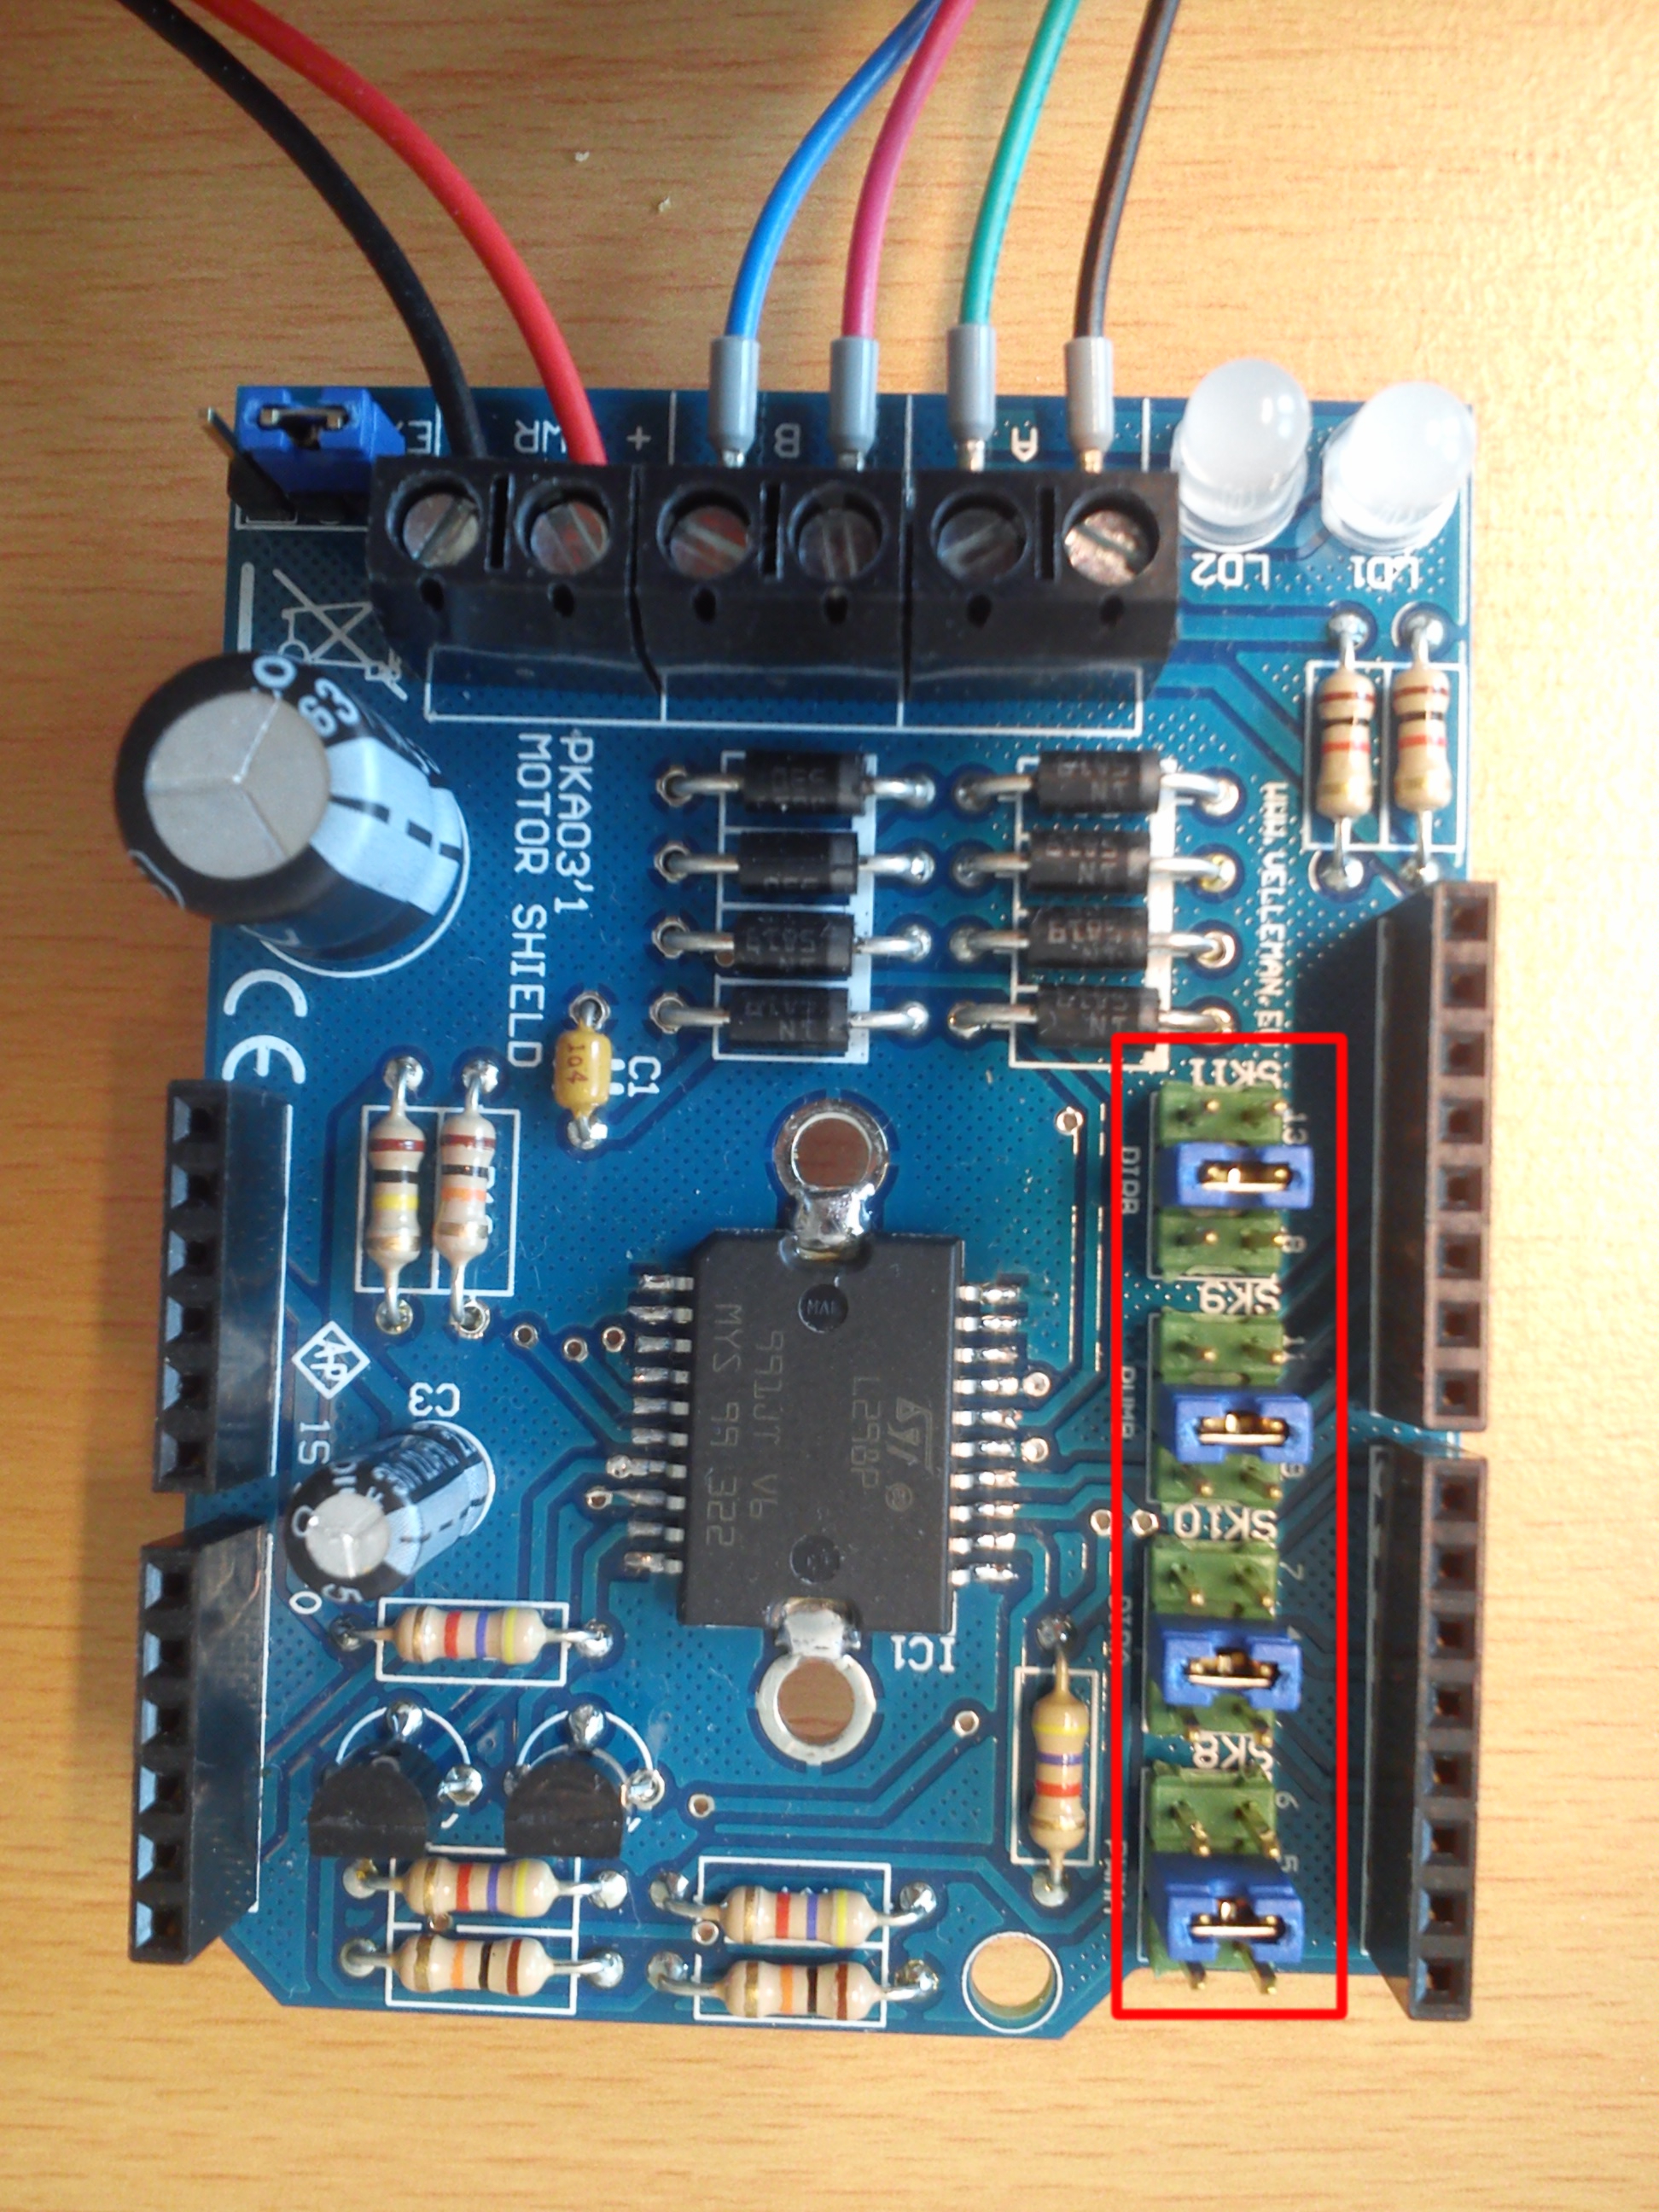
\includegraphics[width=\textwidth]{../figures/motor1.jpg}
        \caption{Motor shield 1}
    \end{subfigure}
    \begin{subfigure}[b]{0.32\textwidth}
      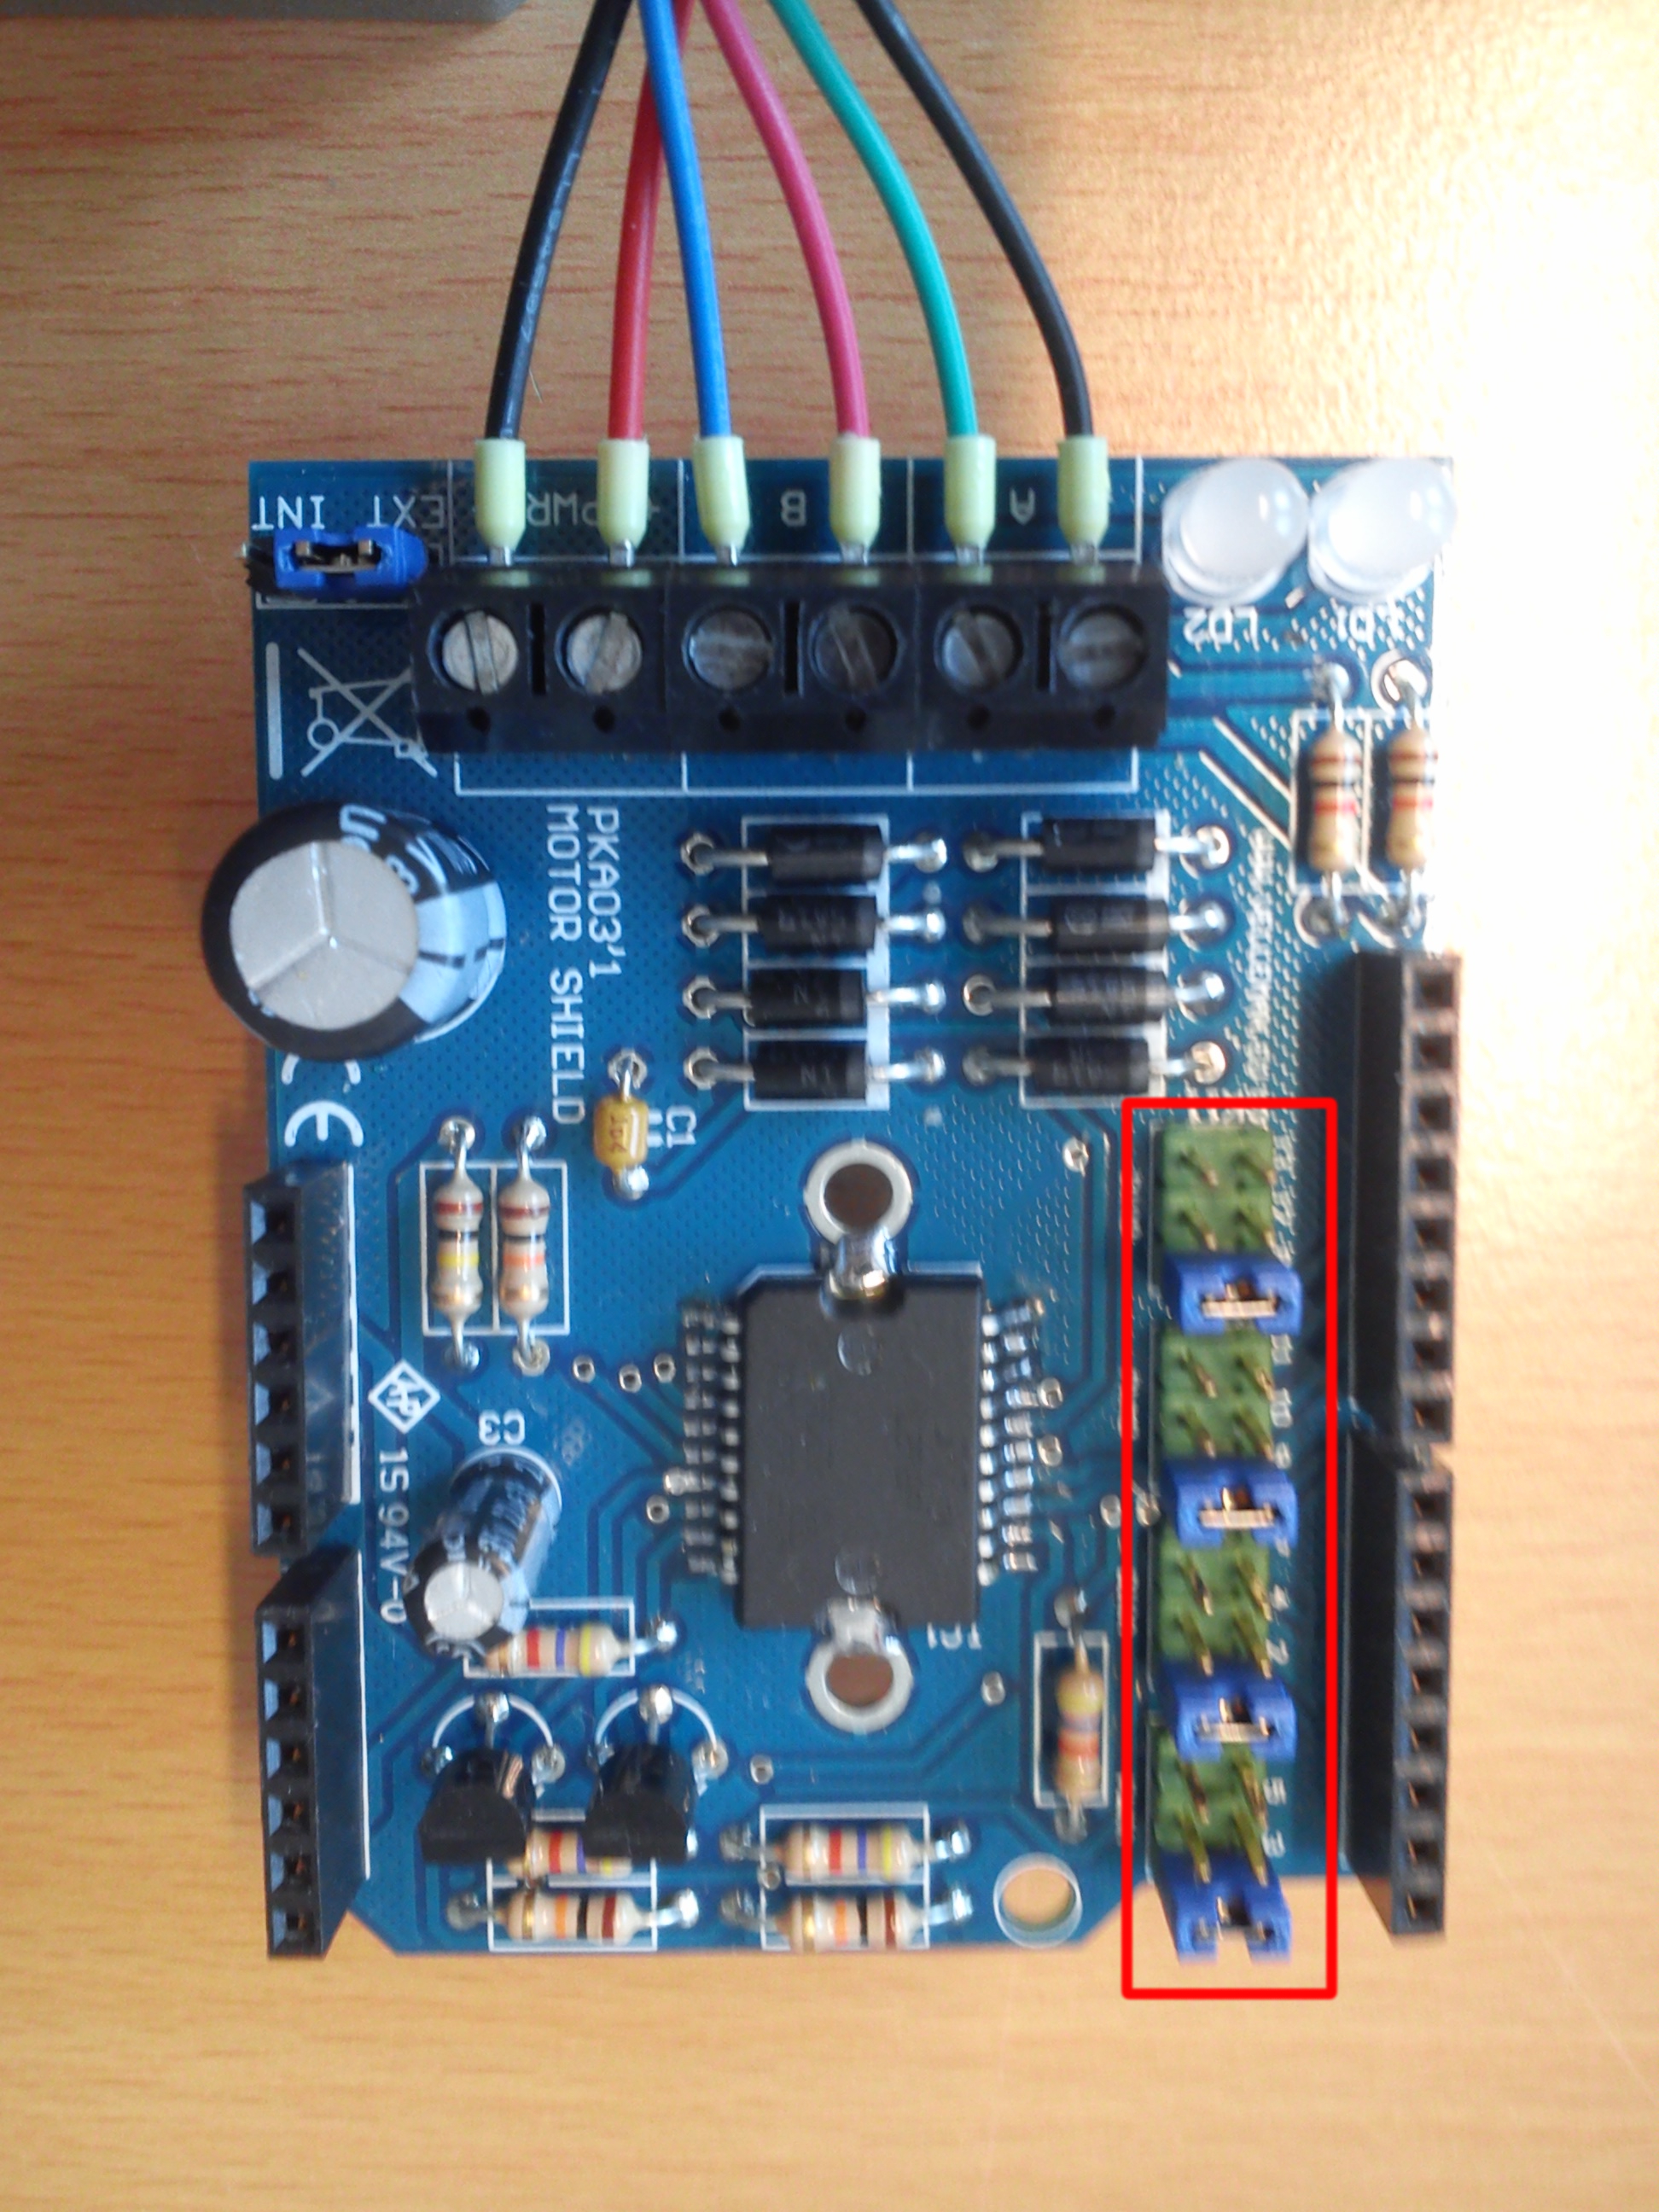
\includegraphics[width=\textwidth]{../figures/motor2.jpg}
        \caption{Motor shield 2}
    \end{subfigure}
  \caption{Components}\label{fig:comp}
\end{figure}

On the top side of the photographs of the motors 6 connections can be seen. The two on the left correspond to the external power supply.
The four on the right correspond to the coils of the motor, a pair for each. A simple way to check which pairs of wires correspond together is to
use the motor as a generator, connecting two wires to a LED (for example). If manually spinning the motor lights
the LED, the wires form a pair.

\section{Controlling the motors}

To move the motor one step in one direction the coils inside the motor have to be alternatively powered on and off. There're two pins controlling the power supplied
to the motor, and two pins controlling the direction. The sequences to move the motor one step in one direction should be:

\begin{table}[here]
\centering 
\begin{minipage}{0.4\textwidth}
  \begin{tabular}{ | c | c | c | c | c |}
    \hline
    \multicolumn{5}{|c|}{clockwise} \\ \hline
      \# & pwr A & pwr B & dir A & dir B \\ \hline
      1 & HIGH & HIGH & LOW & LOW \\ \hline
      2 & LOW & HIGH & LOW & LOW \\ \hline
      3 & HIGH & HIGH & HIGH & LOW \\ \hline
      4 & HIGH & LOW & HIGH & LOW \\ \hline
      5 & HIGH & HIGH & HIGH & HIGH \\ \hline
      6 & LOW & HIGH & LOW & HIGH \\ \hline
      7 & HIGH & HIGH & LOW & HIGH \\ \hline
      8 & HIGH & LOW & LOW & LOW \\
    \hline
  \end{tabular}
\end{minipage}
\hfill
\begin{minipage}{0.4\textwidth}
  \begin{tabular}{ |c | c | c | c | c |}
    \hline
    \multicolumn{5}{|c|}{counter-clockwise} \\ \hline
      \# & pwr A & pwr B & dir A & dir B \\ \hline
      1 & HIGH & HIGH & HIGH & HIGH \\ \hline
      2 & HIGH & LOW & HIHG & LOW \\ \hline
      3 & HIGH & HIGH & HIGH & LOW \\ \hline
      4 & LOW & HIGH & LOW & LOW \\ \hline
      5 & HIGH & HIGH & LOW & LOW \\ \hline
      6 & HIGH & LOW & LOW & LOW \\ \hline
      7 & HIGH & HIGH & LOW & HIGH \\ \hline
      8 & LOW & HIGH & LOW & HIGH \\
    \hline
  \end{tabular}
\end{minipage}

\end{table}


The active pins in the motor shields have to be selected using jumpers. In this setup we choose pins xxxx for xxxx. In figure ref{figure} one can see how the jumpers
should be connected for the setup to work.

\begin{lstlisting}
//motorV - shield 1
const int pwr_aV = 3;
const int pwr_bV = 9;
const int dir_aV = 2;
const int dir_bV = 8;

//motorH - shield 2
const int pwr_aH = 5;
const int pwr_bH = 10;
const int dir_aH = 4;
const int dir_bH = 12;

int servoValV;           
int servoValH;
int nV,nH;

void setup() {
  
  //shield1
  //establish motor direction toggle pins
  pinMode(pwr_aV, OUTPUT); 
  pinMode(pwr_bV, OUTPUT); 
  //establish motor brake pins
  pinMode(dir_aV, OUTPUT); 
  pinMode(dir_bV, OUTPUT); 

  //shield2
  //establish motor direction toggle pins
  pinMode(pwr_aH, OUTPUT); 
  pinMode(pwr_bH, OUTPUT); 
  //establish motor brake pins
  pinMode(dir_aH, OUTPUT); 
  pinMode(dir_bH, OUTPUT); 
  
}

\end{lstlisting}

This is the basic pin assignment and setup. During the loop function the appropiate code to move the motors a certain number of steps read from the serial should be written.
The following is the implementation of the function to move the motor one step in one direction. The variable spd delays the powering of the coils, to make
the movement of the motors faster/slower.

\begin{lstlisting}
void moveFV(int spd){
  
  	digitalWrite(pwr_aV,HIGH);
	digitalWrite(pwr_bV,HIGH);
	digitalWrite(dir_aV,LOW);
	digitalWrite(dir_bV,LOW);
 
	delay(spd);
 
	// Half step (½)
	digitalWrite(pwr_aV,LOW);
	digitalWrite(pwr_bV,HIGH);
	digitalWrite(dir_aV,LOW);
	digitalWrite(dir_bV,LOW);
 
	delay(spd);
 
	// Full step (1)
	digitalWrite(pwr_aV,HIGH);
	digitalWrite(pwr_bV,HIGH);
	digitalWrite(dir_aV,HIGH);
	digitalWrite(dir_bV,LOW);
 
	delay(spd);
 
	// Half step (1½)
	digitalWrite(pwr_aV,HIGH);
	digitalWrite(pwr_bV,LOW);
	digitalWrite(dir_aV,HIGH);
	digitalWrite(dir_bV,LOW);

	delay(spd);

	// Full step (2)
	digitalWrite(pwr_aV,HIGH);
	digitalWrite(pwr_bV,HIGH);
	digitalWrite(dir_aV,HIGH);
	digitalWrite(dir_bV,HIGH);

	delay(spd);

	// Half step (2½)
	digitalWrite(pwr_aV,LOW);
	digitalWrite(pwr_bV,HIGH);
	digitalWrite(dir_aV,LOW);
	digitalWrite(dir_bV,HIGH);

	delay(spd);

	// Full step (3)
	digitalWrite(pwr_aV,HIGH);
	digitalWrite(pwr_bV,HIGH);
	digitalWrite(dir_aV,LOW);
	digitalWrite(dir_bV,HIGH);

	delay(spd);
	// Half step (3½)
        digitalWrite(pwr_aV,HIGH);
	digitalWrite(pwr_bV,LOW);
	digitalWrite(dir_aV,LOW);
	digitalWrite(dir_bV,LOW); 
  
        TurnOffMotors();
 
}
\end{lstlisting}


\section{Thermal camera}

The thermal camera (InfraTec 600 HighResolution) comes with it's own software (IRBIS). This program can control the camera from the PC, focusing, zooming, recording, taking pictures... .
However, it'd be better to be able to control the camera from the command line, or writing a macro, so the process of taking pictures could be automated, and called
from the Arduino macro.

\section{Petalet photos}

The idea is setup the Arduino loop function so it will move the camera over the petalet, stopping at predefined positions.
On each of of those positions the camera should take a photo, and save it. After the last photograph, the camera
should return to the starting position, and the photos should be stichted into a panorama.

\section{Stitching images into a landscape}

\subsection{generating the project file}

The command \textit{pto\_gen} puts a series of jpg files into one project file. For example:
\begin{verbatim}
 pto_gen -o project.pto image1.jpg image2.jpg image3.jpg
\end{verbatim}
will put the selected jpf files into a project called project.pto

\subsection{Generating control points}
\begin{verbatim}
 cpfind --multirow -o project.pto project.pto
\end{verbatim}

\subsection{Pruning control points, image cleaning, final output}
\begin{verbatim}
 cpclean -o project.pto project.pto
 linefind -o project.pto project.pto
 autooptimiser -a -m -l -s -o project.pto project.pto
 pano_modify --canvas=AUTO --crop=AUTO -o project.pto project.pto
 hugin_executor --prefix=prefix project.pto
\end{verbatim}

This will create a project.pto file, which we can use to blend the photos into the final panorama
\begin{verbatim}
 nona -m TIFF_m -o project project.pto
 enblend -o project.tif project0000.tif project0001.tif project0002.tif ...
\end{verbatim}

The template in necessary to sucessfully sticht the photos into a panorama. However, we don't have to repeat this
process for every set of photos covering the petalet. Once we have a template, we can use it to place every
set of photos, assuming they've been taken from the same exact positions.

Once we have a project template, say template.pto, from a previous stichting, we can make a panorama out of a new
set of images this way:
\begin{verbatim}
 nona -o out -m TIFF_m template.pto <ListOfInputImages>
 enblend -o finished.tiff <ListOfTiffsByNona>
\end{verbatim}


\section{questions}

\begin{itemize}
 \item Can a macro be called from Arduino? This would be incredibly useful to integrate into one single process moving the camera, 
 taking the photos and making the panorama
 \begin{itemize}
  \item It's possible using the python library \textit{serial}. The following python script
  \begin{verbatim}
  from time import sleep
  import serial
  from subprocess import call

  ser = serial.Serial('/dev/ttyACM1', 9600) # Establish the connection on a specific port

  while True:
    fromArduino = ser.readline() # Read the newest output from the Arduino
    fromArduino = fromArduino.replace("\n", "")
    if fromArduino == "1":
          call(["ls", "-l"])
  \end{verbatim}
''listens'' to the values written in the Arduino serial. If the value is 1, executes the command ls. In the same way, a macro could
be executed. On the Arduino side, the code looks like:
\begin{verbatim}
  void setup() {
    Serial.begin(9600); // set the baud rate
    Serial.println("Ready"); // print "Ready" once
  }

  void loop() {
    char inByte = ' ';
    if(Serial.available()){ // only send data back if data has been sent
      char inByte = Serial.read(); // read the incoming data
      Serial.println(inByte); // send the data back in a new line so that it is not all one long line
    }
    delay(100); // delay for 1/10 of a second
  }
\end{verbatim}

In this case, arduino prints something on the serial screen. It's this \textit{Serial.println(inByte)} that the python script
is waiting for.

We would have to write to the serial something that the python script would be waiting for. Then, the macro to take
a picture with the camera could be called, for example.

 \end{itemize}

 \item Does the camera save the information corresponding to each pixel, apart from the image? Can we use this information to
 assign different emmisivities to different pixels? (the camera works assuming a single value of the emmisivity for the whole image)
 
\end{itemize}






\end{document}
